\documentclass[UTF8,a4paper,12pt]{ctexart}
\usepackage{geometry}
\usepackage{array}
\usepackage{booktabs}
\usepackage{enumitem}
\usepackage{hyperref}
\usepackage{xcolor}
\usepackage{longtable}
\usepackage{graphicx}
\usepackage{float}
\geometry{left=2.7cm,right=2.7cm,top=2.5cm,bottom=2.5cm}
\hypersetup{colorlinks=true,linkcolor=black,urlcolor=blue}
\setlist{itemsep=3pt,topsep=4pt}

\title{\heiti 清远社区共享地图\\[0.4em]\large 项目介绍}
\author{软件设计大赛参赛项目}
\date{\today}

\begin{document}
\maketitle

\begin{abstract}
清远社区共享地图是一款面向本地居民的 Web 社区地图。项目把地点发现、居民贡献、地图导航和社区评价放在同一个使用场景中，使居民能够方便地找到身边的好去处，也能够把自己熟悉的地点补充到公共地图里。系统采用高德地图作为空间展示与地点核验基础，以 Cloudflare 的边缘服务承载数据和接口，配合登录、审核、评价、私人地图和智能推荐等功能，形成从地点提交到社区使用的完整闭环。
\end{abstract}
\noindent\textbf{关键词：}社区地图；本地生活服务；地图可视化；社区共建；智能推荐

\section{项目背景}

许多本地生活信息分散在聊天记录、短视频评论和个人收藏中。信息能够被看到，却难以持续维护，也不容易按照位置、类别和个人需求重新组织。对于社区居民而言，真正有价值的往往不是一份静态的商家名单，而是一张能够由大家共同补充、核验和使用的生活地图。

清远拥有山水景观、地方美食、商业设施、校园和公共服务资源。项目以清远为实际应用场景，从社区成员的日常需要出发，解决三个问题。第一，地点信息如何以地图方式集中呈现。第二，普通用户如何低门槛提交并维护地点。第三，用户面对大量地点时，如何快速得到符合当前需求的选择。

\section{项目定位与建设目标}

本项目定位为“社区共同维护的本地生活地图”，而不是单纯的地图标注工具。系统既提供浏览和导航，也提供内容生产、质量控制和个人组织能力。

\begin{enumerate}
  \item 建立清远本地地点的统一入口，按景点、美食、商圈、医疗、校园和交通分类管理。
  \item 让居民能够提交地点、补充照片、发表评价和纠正坐标，形成持续更新的社区内容。
  \item 通过高德地点检索和后台审核降低错误地点、重复地点和不当内容的影响。
  \item 以私人地图、协作地图和只读分享满足个人出行与小范围协作需求。
  \item 通过自然语言推荐降低检索成本，在推荐文字之外给出地图高亮和可编辑路线。
\end{enumerate}

\section{主要功能}

\subsection{地图浏览与地点发现}

首页以清远地图为中心展示已经上线的地点。用户可以按分类筛选，按关键词搜索，也可以在最近加入和全部地点页面中浏览。地点列表使用后端分页，搜索和分类筛选直接在数据层完成，避免一次加载全部内容。地点卡片展示封面、评分、点评数量和综合热度，点击后在页面左侧展开详情，地图仍然保留当前定位。

系统记录用户发起导航的次数，并与点赞、点评一起计算综合热度。热度不是单一的点赞数，而是对用户真实使用行为的综合反映。用户可以直接调用高德导航，也可以使用地图上的定位功能查找附近地点。

\subsection{社区提交与内容核验}

登录用户可以提交地点名称、地址、简介、分类和照片。提交时支持地图选点和多图上传，第一张照片作为封面，其余照片进入地点照片墙。后端调用高德 Web 服务对名称、地址和坐标进行核验，能够匹配的地点自动上线，无法确认的内容进入管理后台。

系统对同名同类地点和距离过近的地点进行重复拦截。用户可以在“我的提交”中查看自己提交的地点和审核状态。对于坐标存在偏差的地点，用户可以拖动地图标记提交纠偏建议，由管理员审核后统一生效。

\subsection{评价与社区互动}

登录用户可以点赞、举报和发表点评。每个用户对同一地点保留一条点评，再次提交时更新原有内容。点评可以选择匿名，匿名记录不返回作者字段，其他用户无法据此进入账号主页。实名点评则展示昵称和头像，并可进入该用户公开主页查看非匿名点评。

地点详情页集中展示评分摘要、点评列表和社区照片。照片采用追加方式保存，不会覆盖其他成员已经上传的内容。这样的设计使地点信息从一条提交记录逐步成长为由社区共同维护的内容。

\subsection{私人地图与协作}

用户可以创建多张主题地图，并将地点收藏到指定地图。私人地图支持重命名、查看点位清单、移除点位、顺路规划和只读分享。删除的地图先进入回收站，保留期内可以恢复，过期后自动清理。

地图主人可以按用户名或昵称添加协作者。主人和协作者可以共同维护点位顺序，主人保留删除地图、分享地图和管理成员的权限。只读分享链接只公开地图名称和地点，不暴露创建者和协作者的个人信息。

\subsection{智能推荐与应急服务}

用户可以用自然语言提出“周末带孩子去哪玩”这类需求。系统根据已经上线的地点生成中文推荐，并在主地图和路线小地图上高亮结果。推荐点位按照最近邻原则形成初始游览顺序，用户可以调整顺序、移除地点或添加新的地点，保存后路线会被保留。

系统提供按季节组织的推荐入口，并对相同需求和相近视野进行缓存，减少重复请求。AI 服务设置了超时和备用模型，推荐服务不可用时不会影响地图浏览、地点搜索和其他基础功能。

应急地图可以定位当前位置，并搜索三公里范围内的警察局、医院、消防和避难所。用户可以直接导航或拨打相应电话，也可以向本机保存的预设联系人发送定位信息。联系人数据保存在设备本地，不上传服务器。

\subsection{管理后台}

管理后台包含待审核点位、全部点位、举报处理、账号与密码、位置纠偏和接口诊断六个板块。管理员可以审核地点、修改分类、下架违规内容、处理举报、审批坐标修正和重置用户密码。后台同时提供分类统计和热度排行，便于掌握内容结构。

\section{使用流程}

\begin{enumerate}
  \item 用户打开首页，查看地图、热门地点或最近加入的地点。
  \item 用户通过分类、关键词或当前位置缩小范围，打开地点详情。
  \item 用户可以导航、点赞、点评、收藏，或把地点加入自己的主题地图。
  \item 用户发现新的地点后提交名称、地址、说明和照片，系统进行自动核验。
  \item 对无法自动确认的内容，管理员在后台审核。审核结果同步到公共地图。
  \item 用户通过智能推荐或私人地图组织一次出行，必要时分享只读地图给同伴。
\end{enumerate}

\section{项目特色}

\begin{description}
  \item[内容闭环] 地点提交、地址核验、人工审核、社区评价和纠偏共同构成持续维护机制。
  \item[地图与社区结合] 地图不是信息的终点，用户的照片、评价、导航和收藏都会反过来改善内容排序。
  \item[公共信息与个人组织分离] 公共地点可被社区共同使用，私人地图只保存用户自己的组织方式，分享时只公开必要内容。
  \item[推荐结果可操作] 智能推荐不仅生成文字，还把结果落到地图和路线中，用户可以继续编辑，而不是只能阅读一段答案。
  \item[适合真实部署] 前端为静态页面，后端采用边缘函数和云数据库，部署结构简单，能够以较低成本持续运行。
\end{description}

\section{技术概况}

前端采用原生 HTML、CSS 和 JavaScript，高德地图 JavaScript API 负责地图、定位和地点搜索。后端采用 Cloudflare Pages Functions，以原生 Request 和 Response 提供 JSON 接口。Cloudflare D1 保存地点、用户、评价、私人地图和审核数据，R2 保存图片。高德 Web 服务用于地点检索、地址核验和逆地理编码，智能推荐通过服务端代理调用大模型接口。

\begin{center}
\begin{tabular}{>{\raggedright\arraybackslash}p{3.2cm}p{9.2cm}}
\toprule
组成部分 & 作用 \\
\midrule
Web 前端 & 地图展示、地点浏览、提交、评价、私人地图和推荐交互 \\
Pages Functions & 统一处理认证、地点、评价、地图、管理和推荐接口 \\
D1 数据库 & 保存结构化业务数据，并通过索引支持筛选和分页 \\
R2 对象存储 & 保存地点封面、照片墙和用户头像 \\
高德服务 & 地图显示、地点搜索、地址核验、导航和应急设施查询 \\
AI 服务 & 根据用户需求从已上线地点中生成推荐与初始路线 \\
\bottomrule
\end{tabular}
\end{center}

\begin{figure}[H]
\centering
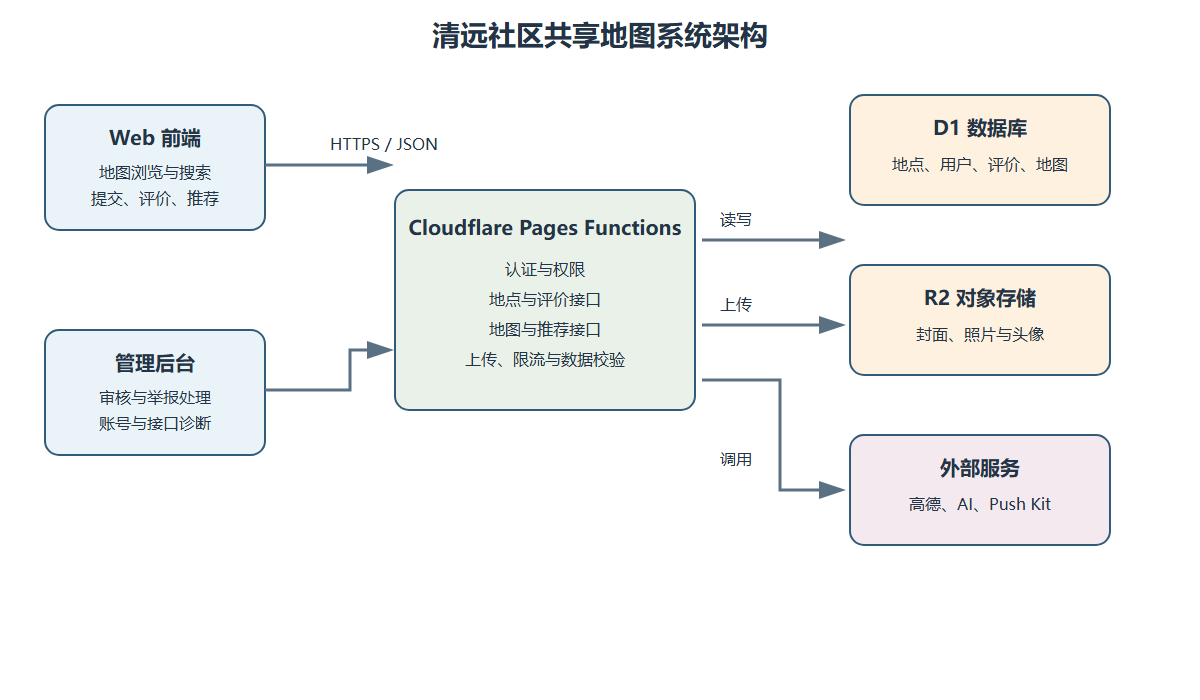
\includegraphics[width=0.94\textwidth]{figures/系统架构图.png}
\caption{系统总体架构}
\end{figure}

\section{应用价值}

项目可以服务于本地居民、返乡青年、游客和社区管理者。居民能够获得更贴近生活的地点信息，游客能够通过公共地图快速了解清远的出行选择，社区成员可以共同维护本地内容，管理者则能够通过审核和举报机制保持信息质量。

从软件设计角度看，项目把地图可视化、内容审核、账号安全、社区协作、云端存储和智能推荐放在同一个完整产品中，既有明确的应用对象，也有可以现场演示的业务闭环。

\section{项目现状与后续完善}

当前版本以 Web 端为参赛主体，已经具备公开地图、地点提交、审核、评价、私人地图、协作、分享、智能推荐和管理后台等功能，并通过 Cloudflare Pages 部署。仓库中同时保留 HarmonyOS 工程，作为后续多端扩展基础。后续可以围绕社区数据增长、推荐效果评估、无障碍体验和移动端深度适配继续完善。

\section{结语}

清远社区共享地图希望解决的不是“地图上再增加几个点”的问题，而是让本地信息能够被发现、被补充、被核验，也能够按照每个人的出行需要重新组织。项目以清远为起点，把社区经验转化为可持续维护的数字地图，为本地生活服务提供一种轻量而实用的实现方式。

\section{典型业务流程}

\begin{figure}[H]
\centering
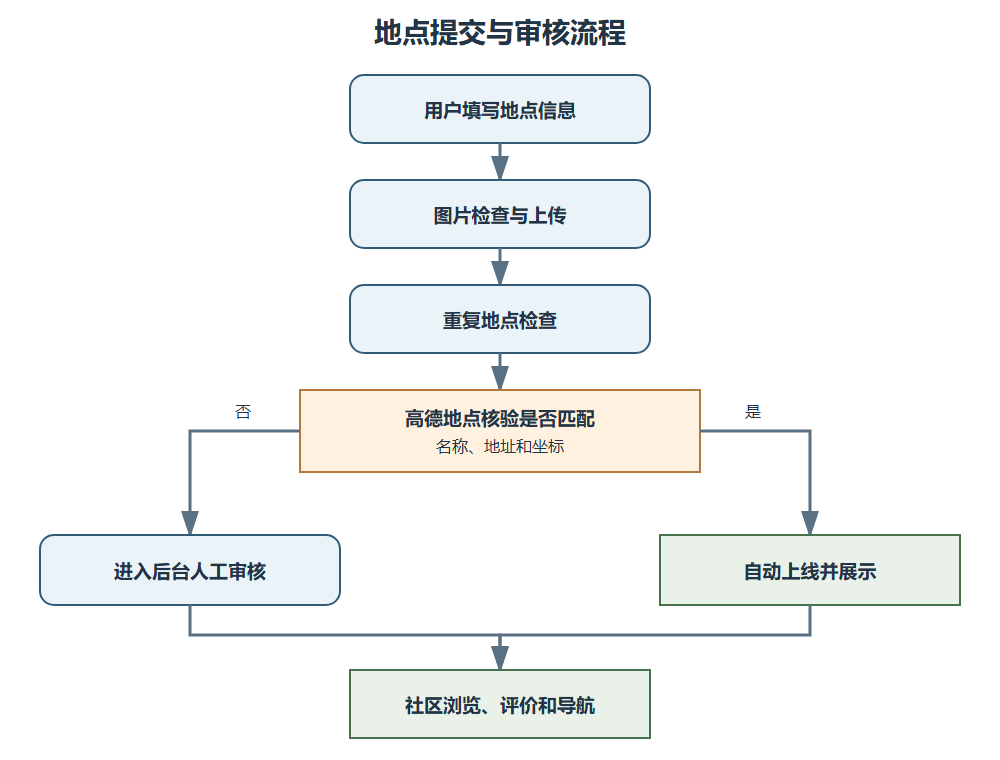
\includegraphics[width=0.98\textwidth]{figures/地点提交流程图.png}
\caption{地点提交与审核流程}
\end{figure}

\begin{figure}[H]
\centering
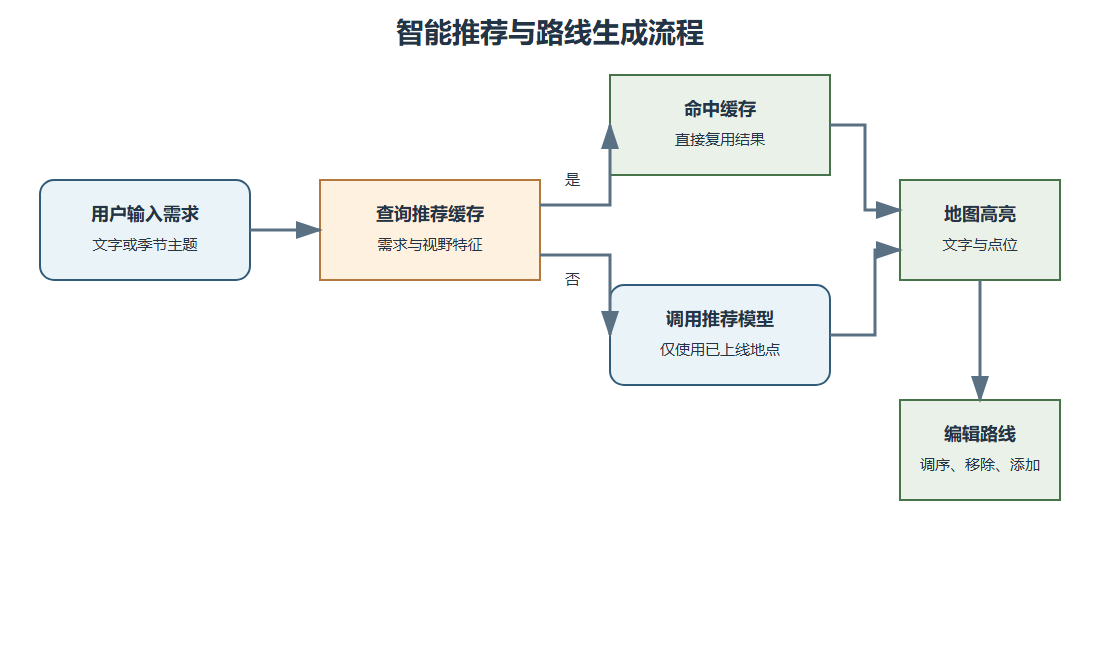
\includegraphics[width=0.98\textwidth]{figures/智能推荐流程图.png}
\caption{智能推荐与路线生成流程}
\end{figure}

\clearpage
\section{系统界面}

以下截图取自当前可访问的 Web 端，选取首页地图和地点浏览页面作为项目代表界面。私人地图模块仍在完善，本材料不将其作为展示内容。

\begin{figure}[H]
\centering
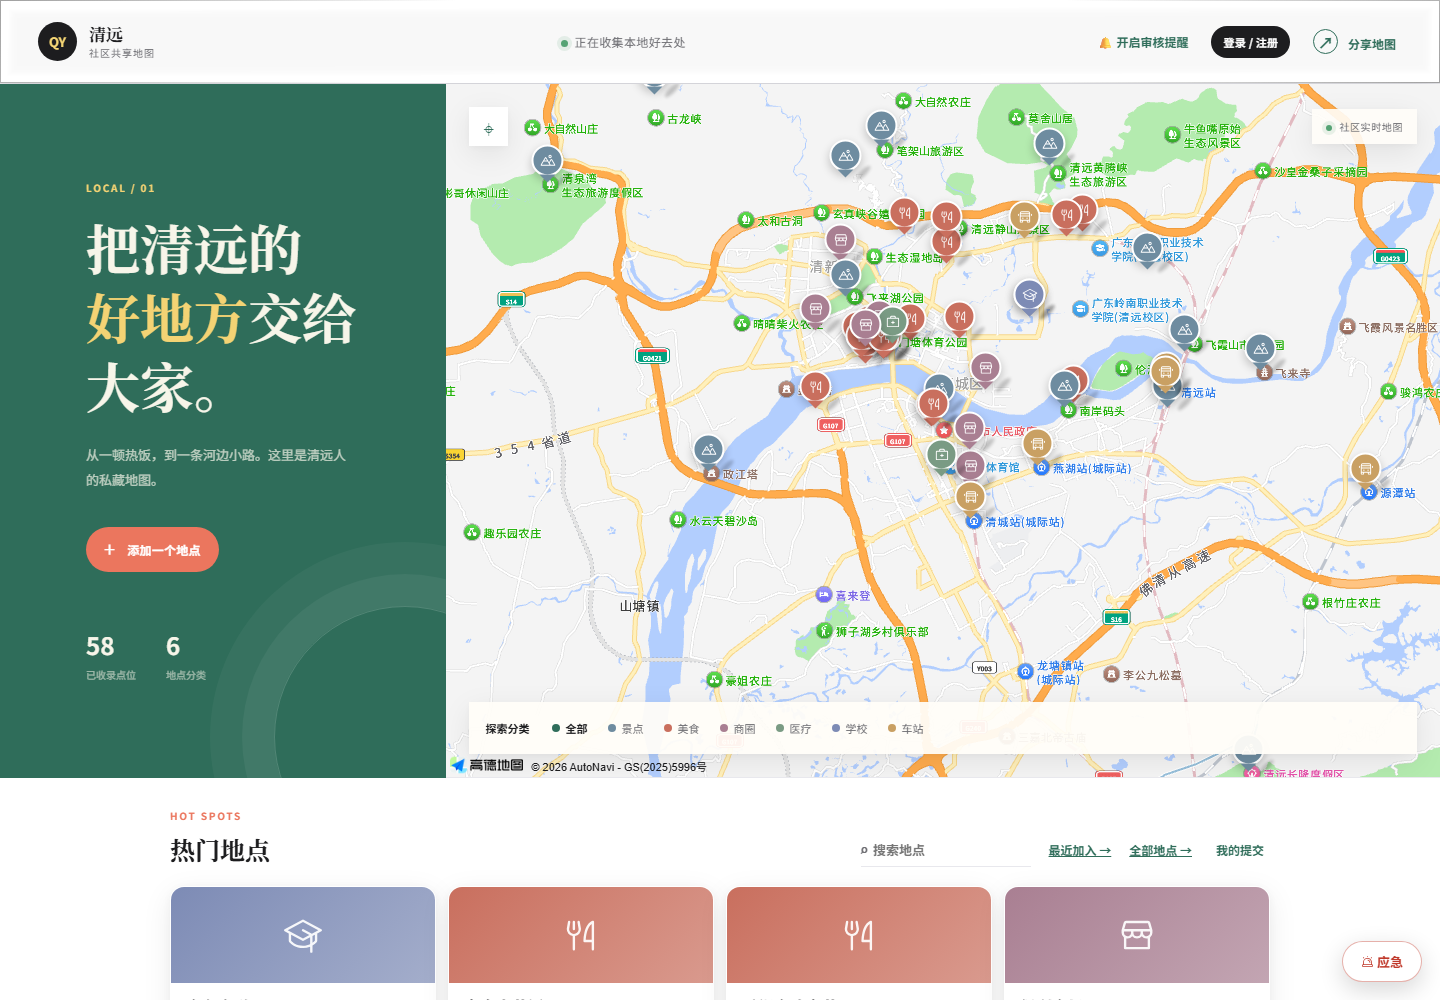
\includegraphics[width=0.98\textwidth]{figures/首页地图.png}
\caption{首页地图与热门地点}
\end{figure}

\begin{figure}[H]
\centering
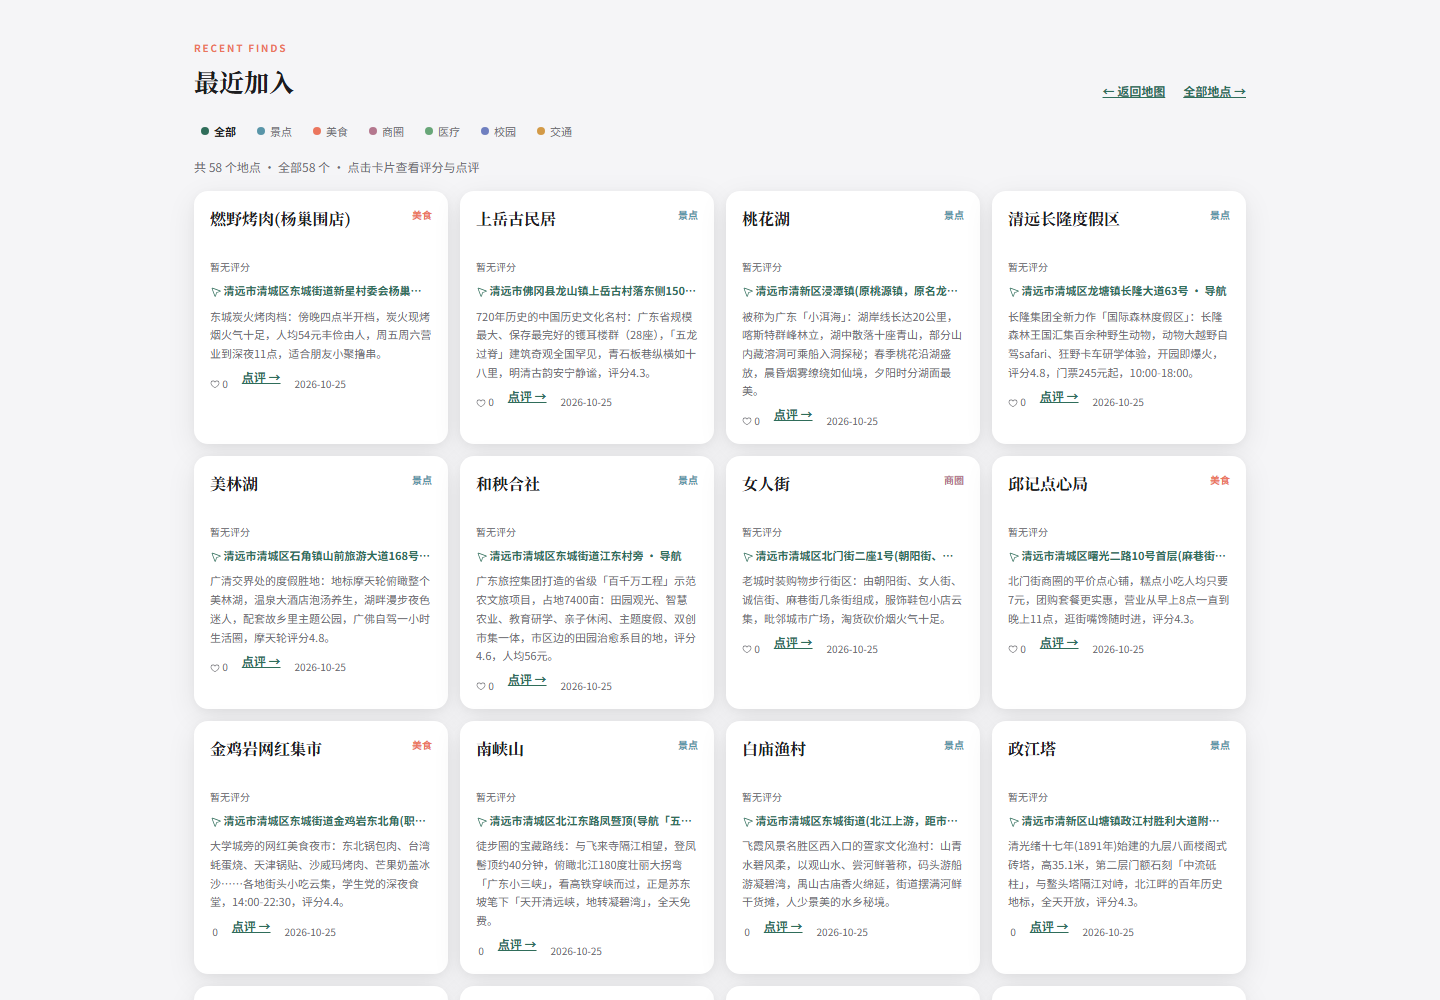
\includegraphics[width=0.98\textwidth]{figures/最近加入.png}
\caption{最近加入地点页面}
\end{figure}

\end{document}
